\section{Výstupní zobrazovací zařízení}
\label{sec:vystupni-zobrazovaci-zarizeni}
Úkolem těchto zařízení je předat informaci uživateli pomocí grafického prostředí.
Do PC je možné tyto zařízení připojit digitálně (HDMI, DisplayPort) či analogově (VGA).
Mezi základní parametry těchto zařízení patří:\\ \\
\begin{tabularx}{\linewidth}{l|l|l}
  \textbf{Parametr}    & \textbf{Jednotka} & \textbf{Popis}                                               \\
  \hline
  Úhlopříčka           & '' (Palce)        & Velikost vzdálenosti mezi protilehlými rohy obrazovky        \\
  \hline
  Rozlišení            & Pixel na pixel    & Počet možných zobrazitelných bodů na výšku a na šířku        \\
  \hline
  Obnovovací frekvence & Hz                & Udává kolikrát za sekundu je obrazovka překreslována         \\
  \hline
  Doba odezvy          & ms                & Udává dobu za kterou se snímek zaslaný na obrazovku vykreslí \\
  \hline
  Spotřeba energie     & W                 & Udává spotřebu energie (Plasma, Crt >> LCD)                  \\
  \hline
  Možnost připojení    & ---               & VGA, DVI, HDMI, DisplayPort, USB-C                           \\
\end{tabularx}
\subsection{Technologie}
Různé technologie využívají jiný způsob zobrazení výsledného obrazu.
Liší se mezi sebou spotřebou, barvama a životností.
\subsubsection{CRT}
Obrazovka monitoru je tvořena velkou elektronkou.
Na jedné straně anoda (obrazovka) a na druhé žhavená katoda (Elektronové dělo).
Vnitřní strana obrazovky je luminofor, který po dopadu elektronu vytvoří světlo.
Pro rosvícení elektronů na správném místě se používá mřížka.
Obraz je vykreslován po řádcích horizntálně vychylován pomocí elektromagnetu.
Obsahuje tři samostatná děla pro každou z barev RGB.
Má vysoký kontrast a dokonalou černou.
Celý monitor je velmi těžký, má vysokou spotřebu a kvůli vypouklé obrazovce zkresluje obraz.
\subsubsection{Plasma}
Jedná se o dvě skleněné desky mezi nimiž leží komůrky s elektrodou se směší plýnů neonu a xenonu.
Po zapnutí elektroda přivede do plynu proud a v plazmě se uvolní volné eketrony.
Poté co se ionty začnou tímto způsobem srážet, tak začnou uvolňovat fotony.
Světlo si takto displej vytváří sám a nepotřebuje k tomu samostatný zdroj.
Na čelní straně každé takové komůrky pak začnou zářit červenou, zelenou nebo modrou barvou.
Na každý pixel jsou takto tři elektrony každý pro jednou barvu.
\subsubsection{LCD}
Technologie tekutých krystalů.
Chemická látka pod vlivem elektrického pole mění svojí molekulární strukturu podle které určují množství procházející světla.
Chová se jako kapamtila ale optické vlastnosti má krystalických látek, je složena z podlouhlých molekul orientovaných v jednom směru.
Každý pixel se skládá z molekul takových tekutých krystalů mezi dvěma elektrodami a polarizačními filtry.
Osy filtrů jsou na sebe kolmé.
Bez krystalů by světlo prošlo jedním filtrem, ale bylo by blokováno druhým.
Světlo je generováno pomocí buďto pasivního (Venkovní světlo) nebo aktivního zdroje světla za krystaly (LED).
Každý pixel je rozdělen na tři subpixely pro RGB.
Používají se dvě technolgie:\\
\begin{description}
  \item[TN]- Světlo bez natočení krystalů projde. Starší technologie.
  \item[IPS]- Světlo bez natočen krystalů neprojde. Novější technologie. Lepší barvy a pozorovací úhly.
\end{description}
\subsubsection{OLED}
Technologie organických (založené na uhlíku) elektroluminiscenčních diod.
Po zavedení proudu diody vyzařují světlo.
Možnost využití pro tenký a pružný displej, ejlikož mezi anodou a katodou je luminofor, který po průchodu elektronů vyzařuje fotony.
Má široké pozorovací úhly, vysoký jas, rychlou odezvu, dobrý konstrast a skutečnou černou barvu.
Má menší životnost oproti LCD a může dojít k vypálení obrazovky.
\subsubsection{Projektory}
Zařízení které zobrazuje obraz na ploše nikoly na displayi.
Využívá pro velké místnosti, jelikož jsme takto jednoduše schopni zobrazit obraz i na metrové plochy.
Existují dva druhy projektorů.
Buďto bílé světlo z lampy dopadá pomocí rotujícího kotouše na soustavu poloprostustných zdrcadel nebo projektor obsahuje tři LCD displeje, každý pro barvu jednu RGB, který potom pomocí optické soustavy promítá.
LCD má větší ostrost obrazu.\\
\begin{multicols}{2}
  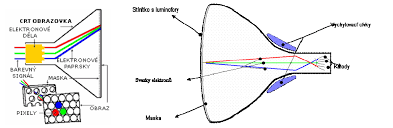
\includegraphics[width=\linewidth]{TVY-POS/Vystupni-zobrazovaci-zarizeni/crt.png}
  \columnbreak
  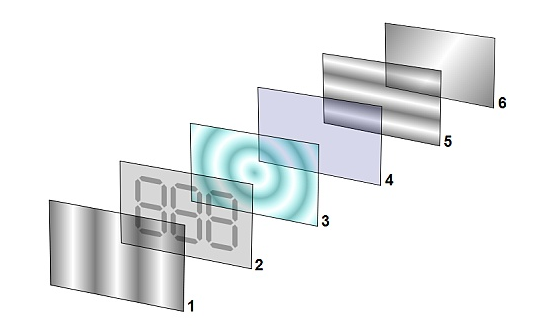
\includegraphics[width=\linewidth]{TVY-POS/Vystupni-zobrazovaci-zarizeni/lcd.png}
\end{multicols}
\begin{multicols}{2}
  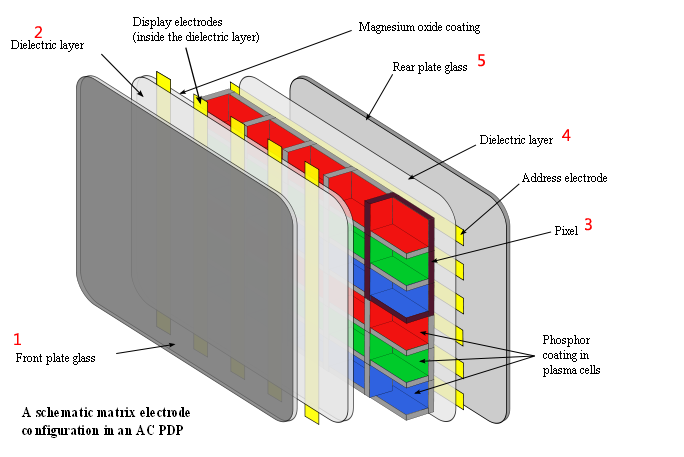
\includegraphics[width=\linewidth]{TVY-POS/Vystupni-zobrazovaci-zarizeni/plasma.png}
  \columnbreak
  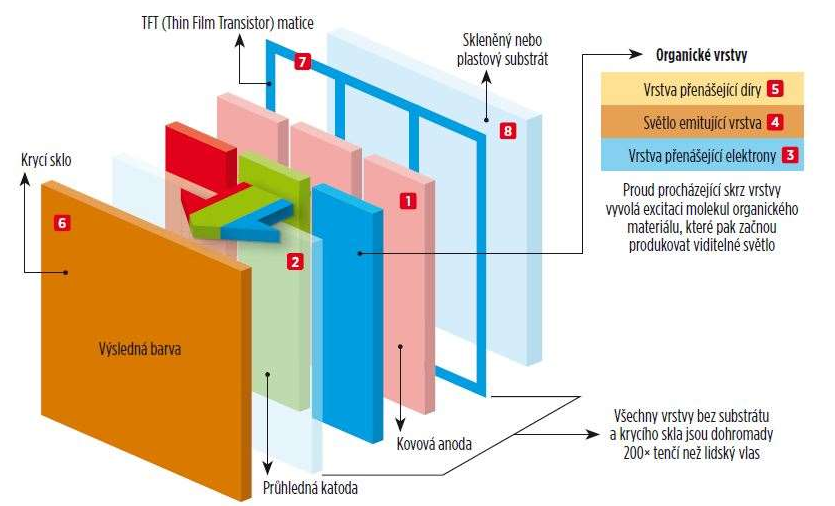
\includegraphics[width=\linewidth]{TVY-POS/Vystupni-zobrazovaci-zarizeni/oled.png}
\end{multicols}
\begin{center}
  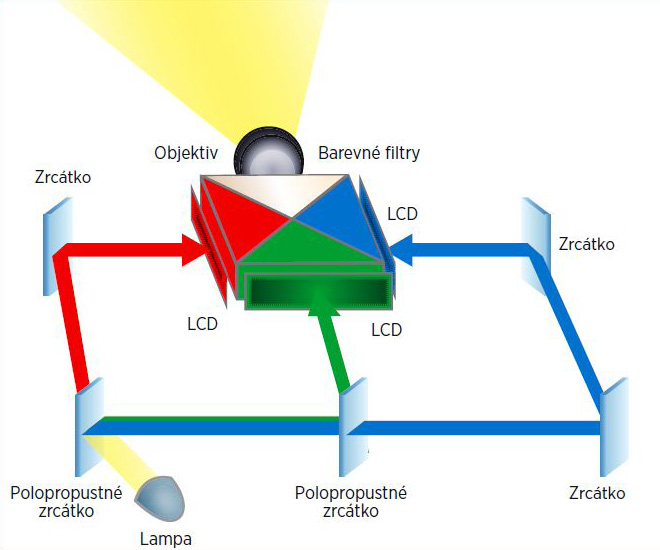
\includegraphics[width=0.5\linewidth]{TVY-POS/Vystupni-zobrazovaci-zarizeni/lcd-projektor.jpg}
\end{center}
